\documentclass[11pt]{jsarticle}
\usepackage{amsmath, amsthm, amssymb}
\usepackage[dvipdfmx]{graphicx}
%\usepackage{eclbkbox}
% \usepackage{listings}
\usepackage{verbatim}
\usepackage{ascmac}
\usepackage[dvipdfmx,svgnames]{xcolor}%tikz$B%Q%C%1!<%8$h$j$bA0$KFI$_9~$_$^$9!#(B%
\usepackage{tikz}
% \usepackage{siunitx}

\usetikzlibrary{arrows}
\usetikzlibrary{intersections, calc}
\usetikzlibrary{patterns}
% \usetikzlibrary{arrows.meta}
\usetikzlibrary{datavisualization}
\usetikzlibrary{intersections,calc}%$B8rE@$r5a$a$k!$:BI87W;;(B
\usetikzlibrary{angles}


\title{Tikz $B%5%s%W%k(B}
\author{$BBk9g9'G7(B}

\begin{document}

\maketitle

\everymath{\displaystyle}

\section{$B$O$8$a$K(B}
\subsection{$B3F?^7A$N=q<0$K$D$$$F$N4JC1$J@bL@(B}

\begin{enumerate}
  \item $BJ}4c$N=q<0(B
  \begin{itemize}
    \item $BJ}4c$O(B \textbackslash draw ($B:82<6y(B) grid ($B1&>e6y(B);
      \begin{itemize}
        \item $B%*%W%7%g%s$N(B[help lines]$B$K$h$C$F!$J}4c$,%0%l!<$N:Y@~$K$J$k(B
        \item $B$5$i$K(B[step = 5mm]$B$J$I$H$7$FJ}4c$N4V3V$r@_Dj$G$-$k!J%G%U%)%k%H$G$O(B1cm$B!K(B
      \end{itemize}
  \end{itemize}       
  \item $BD>@~$N=q<0(B
    \begin{itemize}
     \item $B@~J,$O(B\textbackslash draw ($B;OE@(B) -- ($BCf4VE@(B) $B!D(B -- ($B=*E@(B);
           \begin{itemize}
            \item $BE@$HE@$N$"$$$@$N(B--$B$O!V%O%$%U%s(B2$B8D!W(B
            \item $B%Q%9$rJD$8$k$H$-$O:G8e$K(B --cycle $B$r$D$1$k!J$3$N%*%W%7%g%s$G;OE@$KLa$k$3$H$K$J$k!K(B
            \item $B3j$i$+$J3Q$K$9$k$K$O$=$N<jA0$G(B [rounded corners] -- $B$H$9$k(B
            \item $B:F$SD>@~E*$J3Q$K$9$k$K$O$=$N<jA0$G(B [sharp corners] -- $B$H$9$k(B
            \item ($B=*E@(B) $B$N:BI8$r6K:BI87A<0(B ($B3QEY(B:$BD9$5(B)$B$GI=8=$9$k$3$H$b$G$-!$(B++$B$r$D$1$l$P;OE@$+$i$NAjBP:BI8$H$J$k!J$J$1$l$P@dBP:BI8!K(B

           \end{itemize}
     \item $BD9J}7A$O(B \textbackslash draw ($B:82<6y(B) rectangle ($B1&>e6y(B);
     \item $B%?%F!&%h%3$@$1$G7k$V@~$O(B \textbackslash draw ($B;OE@(B) |- ($B=*E@(B); $B$^$?$O(B
           \textbackslash draw ($B;OE@(B) -| ($B=*E@(B);
           \begin{itemize}
            \item "--"$B$,(B ($B;OE@(B) $B$H(B ($B=*E@(B)$B$r$^$C$9$0$K7k$V$N$KBP$7!$(B|-$B$O!V;O$a$K%?%F!$<!$K%h%3!W$G(B2$BE@$r(B
                  $B7k$S!$(B-|$B$O!V;O$a$K%h%3!$<!$K%?%F!W$G(B2$BE@$r7k$V(B
           \end{itemize}
    \end{itemize}
 \item $B1_!$BJ1_!$8L!J@p7A!K$N=q<0(B
       \begin{itemize}
        \item $B1_$O(B \textbackslash draw ($BCf?4(B) circle [radius=r];
       \begin{itemize}
        \item $B8E$$;EMM$G$O!$H>7B$r(B(r)$B$H$D$1$k$3$H$K$J$C$F$$$?$,!$2DFI@-$N4QE@$+$i:BI80J30$r(B
               ( )$B$G0O$`$3$H$O8=:_$O?d>)$5$l$F$$$J$$(B
        \item $B:BI8>e$N!VE@!W$r9u4]$G<($9$H$-$K$O5l7A<0$NI=5-$,$h$/MQ$$$i$l$k(B
              $B!J(B\textbackslash fill ($BCf?4(B) circle (2pt);$B!K(B
       \end{itemize}
        \item $BBJ1_$O(B \textbackslash draw ($BCf?4(B) circle [x radius = x$BJ}8~$N7B(B, y radius = y$BJ}8~$N7B(B,
              rotate = $B2sE>3Q(B];
              \begin{itemize}
               \item $B2sE>3Q$O%i%8%"%s!J8LEYK!!K$G$O$J$/!$EY?tK!!J(B1$B2s(B
                     $BE>$,(B360$BEY$H$J$k$b$N!K$GI=$9(B
              \end{itemize}
        \item $B8L$O(B \textbackslash draw ($B;OE@(B) arc
              [start angle = $B;OE@$N3QEY(B, end angle = $B=*E@$N3QEY(B, radius = $BH>7B(B];
              \begin{itemize}
        \item $B3QEY$O%i%8%"%s!J8LEYK!!K$G$O$J$/!$EY?tK!!J(B1$B2sE>$,(B360$BEY$H$J$k$b$N!K$GI=$9(B
        \item $BN,<0$G$O(B \textbackslash draw ($B;OE@(B) arc ($B;OE@$N3QEY(B:$B=*E@$N(B
              $B3QEY(B:$BH>7B(B); $B$H$9$k$3$H$b$G$-$k(B
        \item $B;OE@$N3QEY$^$?$O=*E@$N3QEY$N0lJ}$NBe$o$j$K(B delta angle = $BCf?43Q(B $B$r@_Dj$9$k$3$H$b$G$-$k(B
        \item radius $B$NBe$o$j$K(B x radius $B$H(B y radius $B$K0[$J$C$?D9$5$r@_Dj$9$l$PBJ1_$N8L$N0lIt$K$J$k(B
              \end{itemize}
       \end{itemize}

 \item $BJ|J*@~!$%5%$%s%+!<%V!$6J@~!$%Y%8%'6J@~$N=q<0(B
       \begin{itemize}
        \item $BJ|J*@~$O(B \textbackslash draw ($B;OE@(B) parabola bend ($BD:E@(B) ($B=*E@(B);
              \begin{itemize}
               \item $B$?$@$7!$>e$N<0$O!V;OE@$+$iD:E@$^$G$NJ|J*@~!W$H!VD:E@$+$i=*E@$^$G$NJ|J*@~!W$rI=$7!$(B
                     $BI,$:$7$b(B3$BE@$rDL$k(B1$B$D$NJ|J*@~$K$J$k$H$O8B$i$J$$(B
                     $B!JF10lJ|J*@~$K$9$k$K$O!$E,@Z$J:BI8$r5-=R<T<+?H$,M?$($J$/$F$O$J$i$J$$!K(B
               \item \textbackslash draw ($B;OE@(B) parabola ($B=*E@(B); $B$H(B2$BE@$N$_$rM?$($?>l9g$O;OE@$,D:E@!$(B
                     \textbackslash draw ($B;OE@(B) parabola [bend at end] ($B=*E@(B)$B$H$7$?>l9g$O=*E@$,D:E@$K$J$k(B
               \item \textbackslash draw ($B;OE@(B) parabola [parabola height = $B9b$5(B] +($BI}(B,0);
              \end{itemize}
        \item $B%5%$%s%+!<%V$O(B \textbackslash draw ($B;OE@(B) sin ($BD:E@(B); $B$^$?$O(B \textbackslash draw ($BD:E@(B) cos ($B=*E@(B);
              \begin{itemize}
               \item sin$B$rMQ$$$l$P!V86E@$+$iD:E@$^$G!W$N(B1/4$B<~4|$rIA$-!$(Bcos$B$rMQ$$$l$P(B
                     $B!VD:E@$+$i86E@$^$G!W$N(B1/4$B<~4|$rIA$/!J$$$:$l$b(B[0, $B&P(B/2]$B$NHO0O$H$$$&$3$H!K(B
               \item $B;03Q4X?t$N(B1$B<~4|J,$r5-=R$9$k$K$O!$(Bsin $B$H(B cos $B$rE,@Z$KAH$_9g$o$;$k(B
               \item sin $B$*$h$S(B cos $B$GIA$+$l$k$N$O;03Q4X?t$N(B1/4$B<~4|J,$N$_(B
              \end{itemize}
        \item $B6J@~$H$7$F(B \textbackslash draw ($B;OE@(B) to [out = $B;OE@$+$i=P$k3QEY(B, in = $B=*E@$KF~$k3QEY(B] ($B=*E@(B);
              \begin{itemize}
               \item 2$BE@$N!V=P!W$H!VF~$j!W$N3QEY$r;XDj$7!$3j$i$+$J6J@~$G$D$J$0(B
               \item {[out = $B!{(B, in = $B!{(B]} $B$H$$$&%*%W%7%g%s$,$J$1$l$P!$(B
                     $B>e<0$O(B \textbackslash draw ($B;OE@(B) -- ($B=*E@(B); $B$KEy$7$$(B
              \end{itemize}
        \item {[bend $BJ}8~(B (= $B3QEY!K(B, distance = $B5wN%(B]} $B$H$$$&%*%W%7%g%s$G(B2$BE@4V$r4K$d$+$KKD$i$s$@6J@~$G7k$V(B
              \begin{itemize}
               \item $BJ}8~$O!J?J9TJ}8~$KBP$7$F!K(B left $B$^$?$O(B right
               \item $B3QEY$r;XDj$9$k$H(B [out = $B3QEY(B, in = 180 - $B3QEY(B ] $B$r0UL#$9$k(B
               \item $B3QEY$r>JN,$9$k$H!$0JA0$N?tCM$,5!3#E*$K;H$o$l$k(B
               \item distance $B$GKD$i$_6q9g$rD4@0$G$-$k!J%Y%8%'6J@~$N(B controls $B$N5wN%$rD4@0$7$F$$$k!K(B
              \end{itemize}
        \item $B%Y%8%'6J@~$O(B \textbackslash draw ($B;OE@(B) .. controls ($BJ}8~E@(B1) and ($BJ}8~E@(B2) .. ($B=*E@(B);
              \begin{itemize}
               \item 3$B<!$N%Y%8%'6J@~$K$J$k(B
               \item $BJ}8~E@(B2$B$r>JN,$9$k$H!$J}8~E@(B2$B$H=*E@$,0lCW$7$F$$$k$H8+$J$5$l$FIA2h$5$l$k(B
              \end{itemize}
       \end{itemize}
 \item $B4X?t$K$h$kIA2h(B
       \begin{itemize}
        \item $B:BI8;XDj$N(B y $B:BI8$,(B x $B:BI8!J(B\textbackslash x$B!K$N4X?t$K$J$k$h$&$K5-=R$9$k(B
              \begin{itemize}
               \item $B%G%U%)%k%H$NJQ?t$O(B \textbackslash x $B$@$,!$(B
                     $B%*%W%7%g%s$G(B variable = \textbackslash t $B$J$I$H$9$l$PJQ$($i$l$k(B
               \item $BJQ0h$N%G%U%)%k%H$O(B[-5:5]$B$@$,!$%*%W%7%g%s$G(B domain = <start>:<end> $B$H;XDj$G$-$k(B
               \item $BI,MW$K1~$8$FCf3g8L!J(B{, }$B!K$r;HMQ$9$k(B
              \end{itemize}
        \item $B$3$3$G$O(B PGF (TikZ) $B$N7W;;5!G=$rMxMQ$7$F$$$k!J(Bgnuplot $B$J$I$N30It%(%s%8%s$NMxMQ$b2DG=!K(B
              \begin{itemize}
               \item $B;HMQ2DG=$J(B PGF $B$N7W;;5!G=$K$D$$$F$O%^%K%e%"%k$NBh(B89$B>O(B Mathematical Expressions $B$r;2>H(B
              \end{itemize}
       \end{itemize}
\end{enumerate}

\newpage

\section{$BNc(B}

\subsection{$B:BI8<4(B}

\begin{minipage}[t]{0.5\textwidth}
 % \vspace{0zw}
  \begin{itembox}[l]{LaTeX}
 {\scriptsize
    \verbatiminput{manual01-axes01.tex}
 }
 \end{itembox}
\end{minipage}
\begin{minipage}[t]{0.5\textwidth}
 \vspace{0zw}
  \begin{center}
   \begin{tikzpicture}
 \datavisualization[
 school book axes,
 x axis={label={$x$}, ticks={major={at={}}}},
 y axis={label={$y$}, ticks={major={at={}}}},
 ]
 data{
 x,y
 -2.5, -2.5
 2.5, 2.5  
 };
  \begin{scope}
   \draw (0,0) node[below left]{O}; % 原点
  \end{scope}
\end{tikzpicture}

  \end{center}
\end{minipage}

\begin{minipage}[t]{0.5\textwidth}
 % \vspace{0zw}
  \begin{itembox}[l]{LaTeX}
 {\scriptsize
    \verbatiminput{manual01-axes02.tex}
 }
 \end{itembox}
\end{minipage}
\begin{minipage}[t]{0.5\textwidth}
 \vspace{0zw}
  \begin{center}
   \begin{tikzpicture}[ > = latex']

\node(O) at (0,0) [below left]{$\mathrm{O}$};
\draw[->] (-3,0) -- (3,0) node[below]{$x$};
\draw[->] (0,-3) -- (0,3) node[left]{$y$};


\end{tikzpicture}

  \end{center}
\end{minipage}
\newpage

\subsection{$B6J@~(B}

% \begin{minipage}[t]{0.5\textwidth}
 % \vspace{0zw}
  \begin{itembox}[l]{LaTeX}
 {\scriptsize
    \verbatiminput{manual01-curve01.tex}
 }
 \end{itembox}
% \end{minipage}
% \begin{minipage}[t]{0.5\textwidth}
%  \vspace{0zw}
  \begin{center}
   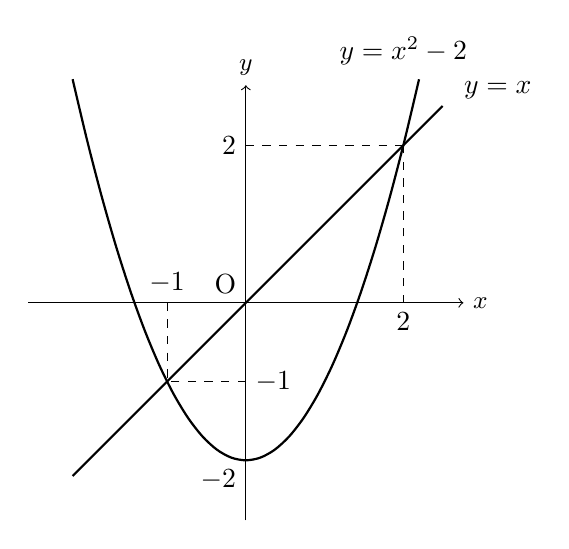
\begin{tikzpicture}
 \datavisualization[
 school book axes,
 x axis={label={$x$},ticks={major={at={}}}},
 y axis={label={$y$},ticks={major={at={}}}},
 ]
 data{
 x,y
 - 2.5, - 2.5
 2.5, 2.5
 };
  \begin{scope}
   \draw (0,0) node[above left]{O};

   \draw[thick, domain=-2.2:2.5] plot (\x,\x) node at(3.2,2.7) {$y = x$};
   \draw[thick, domain=-2.2:2.2,smooth] plot (\x,{\x * \x - 2}) node at(2,3.2) {$y = x^2 -  2$};

   \draw[thin,dashed](2,0) node [below]{$2$}--(2,2);
   \draw[thin,dashed](0,2) node [left]{$2$}--(2,2);
   \draw[thin,dashed](-1,0) node [above]{$ -1$}--(-1, -1);
   \draw[thin,dashed](0, -1) node [right]{$ -1$}--( -1, -1);
   \draw (0, -2) node [below left]{$ -2$};
  \end{scope}
\end{tikzpicture}

  \end{center}
% \end{minipage}

% \begin{minipage}[t]{0.5\textwidth}
 % \vspace{0zw}
  \begin{itembox}[l]{LaTeX}
 {\scriptsize
    \verbatiminput{manual01-curve02.tex}
 }
 \end{itembox}
% \end{minipage}
% \begin{minipage}[t]{0.5\textwidth}
%  \vspace{0zw}
  \begin{center}
   \begin{tikzpicture}[scale = 1.8]
 \datavisualization[
 school book axes,
 x axis={label={$x$},ticks={major={at={}}}},
 y axis={label={$y$},ticks={major={at={}}}},
 ]
 data{
 x,y
 - .5, - .5
 2, 1.5
 };
  \begin{scope}
   \draw (0,0) node[above left]{O};

   \draw[thick, domain=-0:pi/2] plot (\x,{(2/pi) * \x}) node at(2,1.2) {$y = \dfrac{2}{\pi}x$};
   % \draw[thick, domain=-2.2:2.2,smooth] plot (\x,{\x * \x - 2}) node at(2,3.2) {$y = x^2 -  2$};

   \draw[thick] (0, 0) sin (pi/2,1);

   \draw[thin,dashed](pi/2,0) node [below]{$\dfrac{\pi}{2}$}--(pi/2,1);
   \draw[thin,dashed](0,1) node [left]{$1$}--(pi/2,1);

   % \draw (0, -2) node [below left]{$ -2$};
  \end{scope}
\end{tikzpicture}

  \end{center}
% \end{minipage}

\subsection{$BNN0h(B}


% \begin{minipage}[t]{0.5\textwidth}
 % \vspace{0zw}
  \begin{itembox}[l]{LaTeX}
 {\scriptsize
    \verbatiminput{manual01-area01.tex}
 }
 \end{itembox}
% \end{minipage}
% \begin{minipage}[t]{0.5\textwidth}
%  \vspace{0zw}
  \begin{center}
   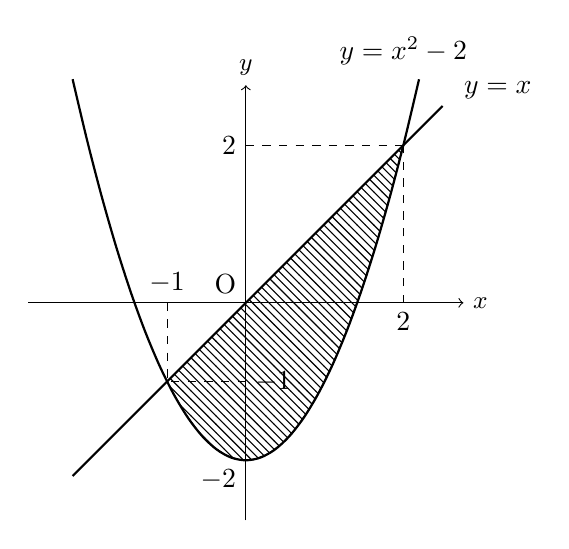
\begin{tikzpicture}
 \datavisualization[
 school book axes,
 x axis={label={$x$},ticks={major={at={}}}},
 y axis={label={$y$},ticks={major={at={}}}},
 ]
 data{
 x,y
 - 2.5, - 2.5
 2.5, 2.5
 };
  \begin{scope}
   \draw (0,0) node[above left]{O};

   \draw[thick, domain=-2.2:2.5] plot (\x,\x) node at(3.2,2.7) {$y = x$};
   \draw[thick, domain=-2.2:2.2,smooth] plot (\x,{\x * \x - 2}) node at(2,3.2) {$y = x^2 -  2$};

   \draw[thin,dashed](2,0) node [below]{$2$}--(2,2);
   \draw[thin,dashed](0,2) node [left]{$2$}--(2,2);
   \draw[thin,dashed](-1,0) node [above]{$ -1$}--(-1, -1);
   \draw[thin,dashed](0, -1) node [right]{$ -1$}--( -1, -1);
   \draw (0, -2) node [below left]{$ -2$};

   \clip (-2.5,-2.5) |- (0, - 2.5) -| (2.5,2.5) --cycle;
   \clip [draw,domain= -2:2.2] plot (\x,{\x * \x - 2});
   \draw [pattern=north west lines](-2.5, -2.5) rectangle (2.5,2.5);
  \end{scope}
\end{tikzpicture}

  \end{center}
% \end{minipage}

\newpage

% \begin{minipage}[t]{0.5\textwidth}
%  \vspace{0zw}
  \begin{itembox}[l]{LaTeX}
 {\scriptsize
    \verbatiminput{manual01-area02.tex}
 }
 \end{itembox}
% \end{minipage}
% \begin{minipage}[t]{0.5\textwidth}
%  \vspace{0zw}
  \begin{center}
   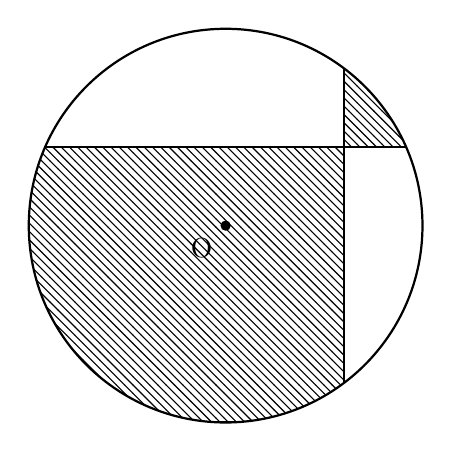
\begin{tikzpicture}[scale=.5]
\path[clip, preaction={draw, thick}] (0,0) circle (5);
\fill[draw=black, thick, pattern=north west lines] (-5,2) -- (3,2) -- (3,-5) -- (-5,-5) -- cycle;

\fill[draw=black, thick, pattern=north west lines] (3,5) -- (3,2) -- (5,2) -- (5,5) -- cycle;
\node[draw, circle, thick, fill=black, minimum size=1mm, inner sep=0, label=225:O] at (0,0) {};
\end{tikzpicture}

  \end{center}
% \end{minipage}

\newpage

\subsection{$B?^7A(B}

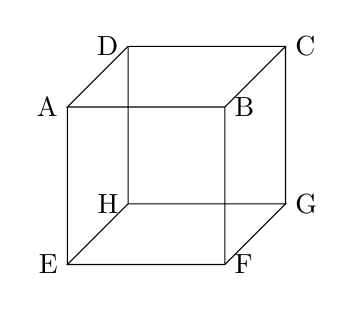
\begin{tikzpicture}
\path
 (0,0,0)  coordinate [label=left:$\mathrm{E}$]  (E)
 (2,0,0)  coordinate [label=right:$\mathrm{F}$] (F)
 (2,2,0)  coordinate [label=right:$\mathrm{B}$] (B)
 (0,2,0)  coordinate [label=left:$\mathrm{A}$]  (A)
 (0,0,-2) coordinate [label=left:$\mathrm{H}$]  (H)
 (2,0,-2) coordinate [label=right:$\mathrm{G}$] (G)
 (2,2,-2) coordinate [label=right:$\mathrm{C}$] (C)
 (0,2,-2) coordinate [label=left:$\mathrm{D}$]  (D)
;

\draw
   (A) -- (B)
       -- (C)
       -- (D) -- cycle
   (E) -- (F)
       -- (G)
       -- (H) -- cycle
   (A) -- (E)
   (B) -- (F)
   (C) -- (G)
   (D) -- (H)
;
\end{tikzpicture}



\newpage




%%%$B3QEY5-9f(B\angmark{A}{O}{B}{$B3QEY(B}
\newcommand{\angmark}[4]{
 \coordinate(Aang)at($(#1)-(#2)$);
 \coordinate(Bang)at($(#3)-(#2)$);
 \draw let \p1=(Aang), \p2=(Bang)
 in ($(#2)!0.5cm!(#1)$) arc
 [start angle={atan2(\x1,\y1)}, end angle={atan2(\x2,\y2)}, radius=0.5cm];
 \draw [opacity=0]
 let \p1=(Aang), \p2=(Bang),
 \n1={atan2(\x1,\y1)}, \n2={atan2(\x2,\y2)}, \n3={0.5*\n1+0.5*\n2}
 in ($(#2)!.8cm!(#1)$)
 arc [start angle={\n1}, end angle={\n3}, radius=.8cm]
 coordinate(Cang);
\draw(Cang)node{#4};}




\begin{tikzpicture}
\coordinate(O)at(0,0)node[above]at(O){O};
\coordinate(A)at(3,-4)node[right]at(A){A};
\coordinate(B)at(-5,-2)node[left]at(B){B};
\draw(A)--(O)--(B);
\angmark{B}{O}{A}{$\theta$}
\end{tikzpicture}


%%%180$B!k$r8Y$03QEY5-9f(B\contrangmark{A}{O}{B}{$B3QEY(B}
\newcommand{\contrangmark}[4]{
 \coordinate(Aang)at($(#1)-(#2)$);
 \coordinate(Bang)at($(#3)-(#2)$);
 \draw
 let \p1=(Aang), \p2=(Bang),
 \n1={atan2(\x1,\y1)}, \n2={atan2(\x2,\y2)+360}
 in ($(#2)!0.5cm!(#1)$)
 arc [start angle={\n1}, end angle={\n2}, radius=0.5cm];
 \draw[opacity=0]
 let \p1=(Aang), \p2=(Bang),
 \n1={atan2(\x1,\y1)}, \n2={atan2(\x2,\y2)+360},
 \n3={0.5*\n1+0.5*\n2}
 in ($(#2)!.8cm!(#1)$)
 arc [start angle={\n1}, end angle={\n3}, radius=.8cm]
 coordinate(Cang);
 \draw(Cang)node{#4};}

 \newcommand{\ang}[1]{#1^\circ}

 \begin{tikzpicture}
\coordinate(O)at(0,0);
\fill(O)circle(2pt);
\coordinate(A)at(120:2)node[above left]at(A){$\ang{120}$};
\coordinate(B)at(200:2)node[below left]at(B){$\ang{200}$};
\draw(O)--(A) (O)--(B);
\contrangmark{A}{O}{B}{$y$}
 \end{tikzpicture}

\newpage

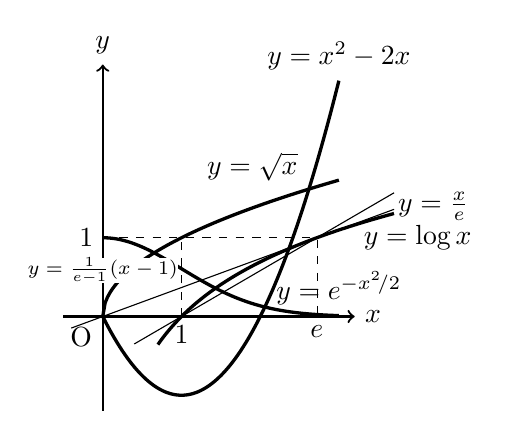
\begin{tikzpicture}[domain=0:3, samples=100, very thick] % $BDj5A0h!"E@$N?t!"@~I}(B
\draw (0,0) node[below left]{O}; % $B86E@!"(B0$B$G$b!"(Babove, below, left, right$B$G0LCV;XDj(B
  % $B0LCV;XDj$O(Banchor=north, south, east, west$B$G$b2DG=(B
\draw[thick, ->] (-0.5,0)--(3.2,0) node[right] {$x$}; % x$B<4!"(B[->]$B$GLp0u!"B>$K(B[-stealth]$BEy(B
\draw[thick, ->] (0,-1.2)--(0,3.2) node[above] {$y$}; % y$B<4(B

\draw plot(\x, {sqrt(\x)}) node at(1.9,1.9) {$y=\sqrt{x}$}; % at$B$G(Bnode$B$N0LCV;XDj(B
\draw plot(\x, \x*\x-2*\x) node[above] {$y=x^2-2x$}; % $BB?9`<0(B
\draw plot(\x, {exp(-0.5 * \x * \x)}) node[above] {$y=e^{-x^2\!/2}$}; % exp

\draw [domain=0.7:3.7] plot(\x, {ln(\x)}); % y=log(x) $BDj5A0h$r8DJL;XDj(B
\node at(4,1) {$y=\log x$};

\draw [thin, domain=-0.4:3.7] plot(\x,\x/e); % y=x/e$B!":Y@~I}(B
\node at(4.2,1.4){$y=\frac{x}{e}$};
\draw [thin, domain=0.4:3.7] plot(\x, {(\x-1)/(e-1)});  % y=(x-1)/(e-1)
\node [above, font=\scriptsize, fill=white, inner sep=0pt] % $BESCf$G2~9T(B
  at(0,0.4){$y=\frac{1}{e-1}(x-1)$}; % node$BDI2C@_Dj(B

\draw [very thin, dashed](0,1) node [left]{$1$}--(e,1)--(e,0) node[below]{$e$}; % $BJd=u@~(B
\draw [very thin, dashed](1,0) node [below]{$1$}--(1,1);
  
\end{tikzpicture}




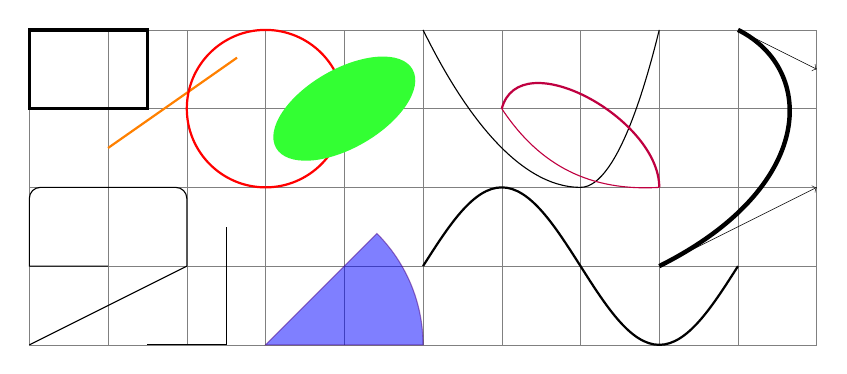
\begin{tikzpicture}
\draw [help lines] (0,0) grid (10,4);%(0,0)$B$+$i(B(10,4)$B$^$G$N(B"$B:Y@~$NJ}4c(B"
%%$BD>@~$NNc(B

\draw (0,0) -- (2,1)  [rounded corners]--(2,2) -- (0,2) [sharp corners] --  (0,1)-- (1,1);
	%$BE@(B(0,0), (2,1), (2,2), (0,2), (0,1), (1,1)$B$r7k$V(B"$B@~J,(B"$B$G!$(B(2,2)$B$H(B(0,2)$B$G$O(B"$B3j$i$+(B"
\draw [orange, thick] (1,2.5) -- ++(35:2cm);
	%(1,2.5)$B$r;OE@$H$7$F(B35$B!k$NJ}8~$K(B2cm$B$N(B"$B%*%l%s%8?'$NB@$$@~J,(B"
\draw [very thick] (0,3) rectangle (1.5,4);
	%(0,3)$B$r:82<!$(B(1.5,4)$B$r1&>e$H$9$k(B"$B6KB@$ND9J}7A(B"
\draw (1.5,0) -| (2.5,1.5);
	%(2,0)$B$H(B(3,1.5)$B$r$^$C$9$07k$P$:$K(B"$B2#@~$H=D@~$N$_$G7k$V(B"
%%$B1_!$BJ1_!$@p7A(B

\draw [red, thick] (3,3) circle (1);
	%(3,3)$B$rCf?4$H$9$kH>7B(B1$B$N(B"$B@V$$B@@~$N1_(B"$B!J8E$$=q<0$G!$8=:_$OHs?d>)!K(B
\fill [green!80] (4,3) circle [x radius=1cm, y radius=5mm, rotate=30];
	%$BCf?4(B(4,3)$B!$2#(B1cm$B!$=D(B5mm$B$N(B"$BBJ1_$r(B30$B!k79$1NP(B80%$B$GEI$C$??^7A(B"$B!J?d>)$5$l$F$$$k?7$7$$1_$N=q<0!K(B
\filldraw [fill=blue, opacity=.5, draw=Indigo] (5,0)  arc (0:45:2) --(3,0)--cycle;
	%(5,0)$B$r=PH/E@$KH>7B(B2$B$N8L$r(B0$B!k$+$i(B45$B!k$^$GIA$-!$(B(3,0)$B$r7PM3$7$F=PH/E@$^$G@~J,$GLa$C$F0O$s$@(B"$BF)L@EY(B50%$B$N@D$GEI$C$?@p7A(B"
%%$BJ|J*@~!$%5%$%s%+!<%V!$6J@~!$%Y%8%'6J@~(B

\draw (5,4) parabola bend (7,2) (8,4);
	%(5,4)$B$r;OE@$H$7(B(7,2)$B$rD:E@$H$9$kJ|J*@~$H(B(7,2)$B$rD:E@$H$7(B(8,4)$B$r=*E@$H$9$k(B"$BJ|J*@~(B"
\draw [thick] (5,1) sin (6,2) cos (7,1) sin (8,0) cos (9,1);
	%(5,1)$B$+$i;O$^$j!$(B(6,2)$B!$(B(8,0)$B$rD:E@$H$7$F(B(9,1)$B$G=*$o$k(B"$BB@@~$N%5%$%s%+!<%V(B"
\draw [purple, thick] (6,3) to [out=75, in=90] (8,2);
	%(6,3)$B$+$i(B75$B!k$N3QEY$G=PH/$7!$(B90$B!k$N3QEY$G=*E@(B(8,3)$B$K;j$k(B"$B;g$NB@$$6J@~(B"
\draw [purple, thin, bend right = 30] (6,3) to (8,2);
	%2$BE@(B(6,3)$B$H(B(8,2)$B$r7k$V(B"$B1&$KKD$i$s$@;g$N:Y$$6J@~(B"$B!J(B30$B!k$N3QEY$G;OE@$r=PH/$7!$(B150$B!k$N3QEY$G=*E@$K;j$k!K(B
\draw [ultra thick] (8,1) .. controls (10,2) and (10,3.5) ..(9,4);
	%$B;OE@(B(8,1)$B!$=*E@(B(9,4)$B$GJ}8~E@$,$=$l$>$l(B(10,2)$B$H(B(10,3)$B$G$"$k(B"$BD66KB@$N(B3$B<!%Y%8%'6J@~(B"
\draw [->, very thin]	(8,1) -- (10,2); \draw[<-, very thin] (10,3.5) -- (9,4);
	%$B>e$N%Y%8%'6J@~$N(B"$B"*$D$-J}8~@~$r<($7$?:Y@~(B"
\end{tikzpicture}




%  \begin{tikzpicture}
%  \draw
%  (3,-1) coordinate (A)
%  -- (0,0) coordinate (B)
%  -- (2,2) coordinate (C)
%  pic["$\alpha$",draw=orange, <->, very thick, angle eccentricity=1.2, angle radius=1cm] {angle=A--B--C};
% %$B@~J,$ND9$5$r<($9Nc(B
%  \draw (B).. controls ($(B)!.2!(C)!10pt!90:(C)$) and ($(B)!.8!(C)!10pt!90:(C)$) .. (C) node [midway, sloped, fill=white] {$a$};
%  \draw (A).. controls ($(A)!.2!(B)!10pt!90:(B)$) and ($(A)!.8!(B)!10pt!90:(B)$) .. (B) node [midway, sloped, fill=white] {$b$};
% \end{tikzpicture}

 
\end{document}
